\documentclass{XDUthesis} %[draft

\title{科学数据的序列分类}
\author{刘精昌}
\date{}
%题目拆分:用于封面
\septitleA{基于\XDUthesis{} 模板的}%如果论文题目长度<=11中文字符只需填此项即可B项空着
\septitleB{论文写作样例}%如果论文题目长度>11中文字符, 建议拆分为10+x or 11+x 将剩余x个字符填在此处。
\class{0712**}%班级号
\schoolnumber{0712****}%学号
\major{统计学}%专业
\school{数学与统计学院}%学院
\supervisor{崔元顺}%指导老师

\begin{document}

% 摘要
% 中文摘要
\begin{abstract}
  本测试样例,供\XDUthesis{} 模板使用者学习之用,会尽量将模板涉及到的命令、环境;以及一些常用的图表、公式排版技巧进行展示,会对参考文献进行进一步阐述。
  
  其余不太重要的部分,会以其他内容进行展示,例如,诗歌、歌词等。

\end{abstract}
\keywords{XDUthesis, 命令, 环境, 排版技巧}

% 英文摘要
\begin{enabstract}
  This paper is just a sample example for the users in learning the \XDUthesis. I will try my best to use the commands and environments which are involved by the \XDUthesis. Also, the popular composition skills in figures, tables and equations will be elaborated.
  
  In the part unimportant, I will show something others, such as poems and lyrics.

\end{enabstract}
\enkeywords{XDUthesis, commands, environments, skills}

% 往PDF属性里面写下关键词信息
\makeatletter
\XDU@setpdf@keywords
\makeatother

\maketitle

% 文章主要部分
\chapter{绪论}
\section{序列以及序列分类}
现实生活中会有各种各样的序列。在语音识别领域,一段语音可以被看作一段序列;在经济领域,股票的走势可以被看作是序列图示;在分子生物学领域,蛋白质、DNA也可以看成是一段序列;在网络管理中,客户端的登录活动也可以被记录成一段序列。而序列分类在现实生活中也有着广泛的应用。以语音库中的不同样本的语音为训练集,通过对需要测试的语音进行分类,可以识别出语音的来源;在医疗领域,通过对心电图序列的分类,可以得到这个疑似患者的患病信息;在信息检索的研究中,利用序列分类可将文件归类;通过蛋白质、DNA序列的分类,有助于科学家探索蛋白质、DNA的新功能\cite{Xing2010}。

一般说来,序列可以看成是事件的集合,而每一个事件可以由符号或者能比较大小的实数表示。比如一段DNA序列可以表示成$ACCCCCGT$,一段简单的时间序列可以表示成$\left\langle {0.2{\rm{,}}0.3{\rm{,}}0.5{\rm{,}}0.9{\rm{,}} \cdots } \right\rangle $,两种序列的不同之处在于实数的大小是可以度量的,而一般而言符号之间的可度量性比较差,本文主要关注的是实数序列。对于符号序列,有一类的处理方法是借鉴实数序列,比如对于蛋白质序列和DNA序列,有一种基于序列对齐的距离度量方法\cite{kajan2006application}。

对于一般的序列分类任务来说,训练集里面的序列都含有描述其类属性的标签。对于语音识别任务来说,语料库里的语音其标签是其发出者;对于文档归类任务来说,文档的标签即是其所属类别。定义$L$为标签集,$S$为待分类序列集,序列分类的任务就是通过对含有标签信息的训练集$T$的训练,得到一个可将$S$映射到$L$的分类器$C$,对于进入$C$中的序列,都能够被贴上一个标签。可以表示成$C:s \to l,s \in S,l \in L$。对于传统的分类任务来说,常用的分类器主要有$k$NN,决策树、支持向量机\cite{Wu2008}。

\section{序列分类的主要方法}
对于序列分类问题,因为其灵活性,很多的学者从不同的角度提出了大量的方法\cite{Al-Naymat2009}\cite{Keogh2000}\cite{Salvador2007}
\cite{Thrun2000}\cite{Xi2006}\cite{Ye2009}。本文主要介绍其中两种比较典型的方法,一种是基于序列距离度量的Dynamic Time Warping(DTW)方法\cite{Al-Naymat2009}\cite{Batista2011}\cite{Keogh2000}\cite{LESLIE2001}\cite{Lin2007}\cite{Salvador2007}
\cite{Xi2006},另一种是基于特征选择的shapelets方法\cite{Ye2009}。其中对DTW方法做重点介绍。

\subsection{DTW方法}
对于分类任务而言,一种广泛使用而且特别简单的方法是$k$NN,使用$k$NN时,关键是度量测试数据和训练数据的亲近与否,也就是需要定义一种距离。对于一般的实数序列,最常用的距离度量是欧氏距离,对于序列$s$和$s^{'}$,它们的欧式距离是:
\begin{equation}\label{equ:1}
  dist\left( {s,{s^{'}}} \right) = \sqrt {\sum\limits_{i = 1}^L {{{\left( {s\left[ i \right] - {s^{'}}\left[ i \right]} \right)}^2}} }
\end{equation}
也就是相同索引的元素的差平方相加再开方。同样地,还可以定义其他诸如街区距离,最大值距离,这里需要重点强调的是,这些距离都是将同索引值元素对齐。

但是对于序列数据而言,这些距离有很大局限性,主要体现在以下两点:
\begin{enumerate}
  \item 以上的距离度量都要求两序列长度相同,而这一点在实际问题中很难得到满足。比如在基因组分析中,很难保证基因序列的长度相同。
  \item 设想这样一种情况。在步态分析中,同一测试者的步速可能不同,或者在某时间段上存在着加速和减速。那么对于其两段步态序列,比较相似的步态之间可能会有一定的时间差,而上面的这些距离测度只会将同一时刻的步态相比较。也就是说,上面的这些距离测度不能反映出序列比较中的错位。
\end{enumerate}

上述的第一个缺点容易克服,两不同长度的时间序列,可以通过插值的方法使得序列等长,从而应用传统的距离度量方法。比如,对于两序列较短的那个,相邻点的之间可插入一定数目的点,插入点的数值可以用这两点的均值代替,以此小技巧,使得短序列扩展到与长序列长度。同样地,分段平均处理能够减小长序列至短序列长度 \cite{Keogh2000}。但是对于对于大多数的序列而言,在描述序列之间的相似性时,更多的是考虑序列形态、走势方面的相似与否,而不会要求相似形态子序列的索引必须一致。传统的距离测度则只会比较同索比较。

DTW方法能够很好地克服上述的两个缺点。

图\ref{fig:1}是DTW示意图,图中的两序列是某一长序列的两段,两子序列之间有一定的索引错位,示意图反映了有错位的两序列的对齐情况\cite{Giorgino2009}。
\begin{figure}[h]
  \centering
  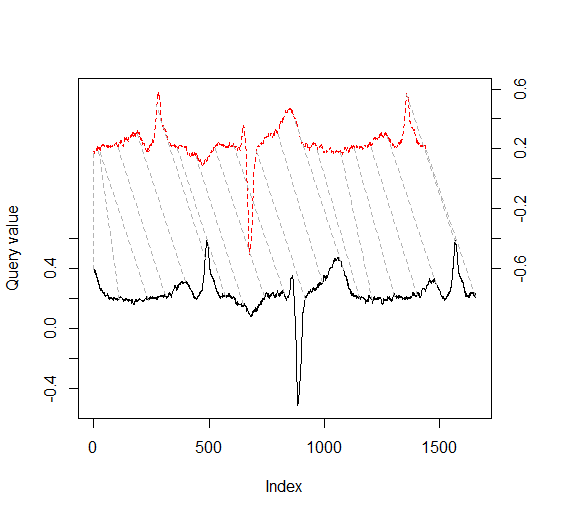
\includegraphics[width=0.6\textwidth]{./figure/two_way_plot.png}
  \caption{DTW示意图}\label{fig:1}
\end{figure}

图中的虚线表示了两序列点的对齐情况,这里对齐的两点指的是用来比较距离的两点,在传统的距离度量中,对齐的两点是索引值相同的两点。而从图中可以看出,对于DTW而言,点的对齐还参考了点邻近曲线的形态,而不仅仅局限于相同索引点,此外序列上的某点可以和另一个序列中的多个点对齐。因而DTW方法还能够直接处理两序列长度不同的情况。DTW的具体求解将在下文中介绍。

\subsection{Shapelets方法}
Shapelets方法最早是由(Ye $et~al$ 2009)提出,作者经过大量实验,验证了该方法的优秀性\cite{Shapelets_website}。

简单来说,选择序列中最能代表该序列的那一部分,比较其与Shapelet的相似度,就可对其分类。最具特征子序列如图\ref{fig:2}所示。

\begin{figure}[t]
  \centering
  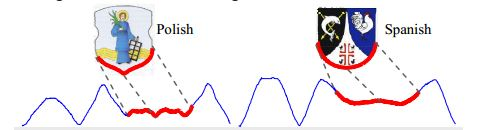
\includegraphics[width=0.6\textwidth]{./figure/shapelets.png}
  \caption{Shapelets示意图}\label{fig:2}
\end{figure}

图中的样本是两个徽章,徽章的边缘可以转换成序列。对于这两个徽章而言,徽章的下部的轮廓最能够反映该徽章的特征,因而可以选择徽章下部轮廓对应的序列,比较其与Shapelet的相似度。可以看出,两徽章的下部明显不同,因而可以由下部序列之间的差异,利用分类器,对徽章进行分类。在这里,一般最常用的分类器是$k$NN分类器,它简单而有效,通常取$k=1$\cite{Xi2006}。如图\ref{fig:3}所示。

\begin{figure}[t]
  \centering
  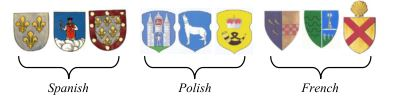
\includegraphics[width=0.6\textwidth]{./figure/shapeletsclassify.JPG}
  \caption{利用Shapelets进行1NN分类示意图}\label{fig:3}
\end{figure}

Shapelets方法有着广泛的应用,比如在植物学中,利用叶柄与叶片的角度,对植物进行分类;在考古学领域,通过对出土器件的特征部位的识别,利用决策树进行分类,能得到考古学发现\cite{anthropology}。如图\ref{fig:4}所示。

\begin{figure}[h]
  \centering
  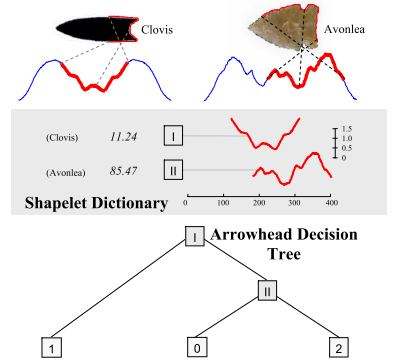
\includegraphics[width=0.6\textwidth]{./figure/anthropology.PNG}
  \caption{基于shapelets的决策树方法对考古器件进行分类}\label{fig:4}
\end{figure}

\chapter{DTW方法的计算以及加速方法}
\section{DTW方法的计算}
\subsection{不带有权重的DTW方法}
首先定义两个序列$Q=q_1,q_2,\cdots,q_i,\cdots,q_m$,$C=c_1,c_2,\cdots,c_j,\cdots,c_n$,并定义$Q$序列的第$i$个元素与$C$序列的第$j$个元素之间的距离为它们的欧式距离,即:
\begin{equation}\label{equ:2}
  D\left( {{i^{th}},{j^{th}}} \right) = d\left( {{q_i},{c_j}} \right) = {\left( {{q_i} - {c_j}} \right)^2}
\end{equation}
DTW方法中很重要的一点就是找到一条从两序列起点,到两序列终点的,能反映两序列对齐关系的warping\ path。下面,首先给出DTW方法的warping\ path的示意图,如图\ref{fig:5}所示。
\begin{figure}[h]
  \centering
  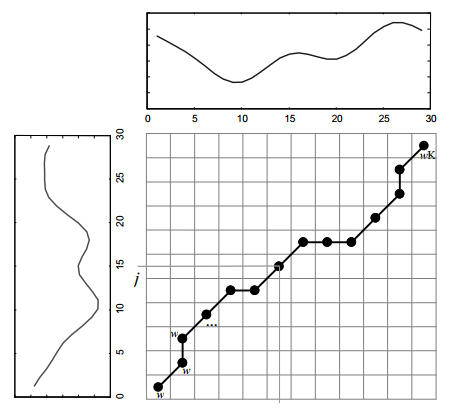
\includegraphics[width=0.5\textwidth]{./figure/three_way_plot.png}
  \caption{warping\ path示意图}\label{fig:5}
\end{figure}
示意图的左方和上方表示两个序列$Q$和$C$,序列之间的方格是能够反映序列对齐关系以及两序列对齐点之间距离信息的度量矩阵$M$,$M$的大小为$m \times n$。$M$中的黑色实线是DTW方法中的warping path。warping path记为
\begin{equation}\label{equ:3}
  W = w_1,w_2,\cdots,w_k,\cdots,w_K \quad max(m,n) \leq K \leq m+n-1
\end{equation}
$w_k$表示路径上的第$k$个点,$w_k={(i,j)}_k$,表示在路径的第$k$步,$q_i$点和$c_j$点进行了对齐。反映在示意图上就是路径的第$k$步经过了$M$的坐标为$(i,j)$的方格。
warping\ path主要有以下三条约束:
\begin{enumerate}
  \item \textbf{Boundary conditions:}\ $w_1=(1,1)$以及$w_K=(m,n)$。这条约束的含义是两序列最开始是起点对齐,最后是两序列的终点对齐。
  \item \textbf{Continuity:}给定路径的第$k$点$w_k=(a,b)$以及路径的第$k-1$点$w_{k-1}=(a^{'},b^{'})$,那么$a-a^{'} \leq 1$ 以及$b-b^{'} \leq 1$。也就是说,路径游走的下一步点只能是当前点周围的那个点而不能跳跃。
  \item \textbf{Monotonicity:}给定路径的第$k$点$w_k=(a,b)$以及路径的第$k-1$点$w_{k-1}=(a^{'},b^{'})$,那么$a-a^{'} \geq 0$ 以及$b-b^{'} \geq 0$。表示路径只能向前游走。
\end{enumerate}

若$w_k=(i,j)$,那么根据上面的三条约束,路径下一步游走的点只能是$w_{k+1}=(i+1,j+1)$或$w_{k+1}=(i+1,j)$或$w_{k+1}=(i,j+1)$。
在这三个约束下,DTW方法需要的优化目标是:
\begin{equation}\label{equ:3}
    DTW(W) = \mathop {\min }\limits_W \left\{ {\sum\limits_{k = 1}^K {d\left( {{w_{ki}},{w_{kj}}} \right)} } \right\}
\end{equation}
$\left( w_{ki},w_{kj} \right)$表示路径$W$上的第$k$个点,说明第$k$步$q_i$和$c_j$点进行了对齐,${d\left( {{w_{ki}},{w_{kj}}} \right)}$表示$q_i$和$c_j$点的距离。也就是说, 路径上的每点都对应着两序列对齐的点之间的距离,现在DTW的目标就是使路径上所有的这样的距离之和最短。
求解这个最小化问题很简单,只需要用贪心的方法,使得每一次的迭代得到的距离和最小即可。定义这样的距离和为累计距离$\gamma(i,j)$。直观意义是路径从距离矩阵的起始位置(左下方)蜿蜒到$(i,j)$方格的最小距离。路径蜿蜒到$(i,j)$方格的上一步是$(i-1,j)$,$(i,j-1)$或$(i-1,j-1)$,因而迭代公式为:
\begin{equation}\label{equ:4}
  \gamma(i,j)=d(q_i,c_j)+\min \left( {\gamma \left( {i - 1,j} \right),\gamma \left( {i,j - 1} \right),\gamma \left( {i - 1,j - 1} \right)} \right)
\end{equation}
根据这个迭代公式,DTW方法的伪代码如\ Algorithm\ref{Alg1}所示。

\algsetup{linenosize = \tiny,
    linenodelimiter=.}
\begin{algorithm}[h]
\caption{Calculate DTW}
\begin{algorithmic}[1]
\small
\REQUIRE $Q:array[1..m], C:array[1..n]$
\ENSURE $DTW[m,n]$

\STATE $DTW := [0..m,0..n]$
\FOR{$i:=0$ to $m$}
\STATE $DTW[i,0] := inf$
\ENDFOR
\FOR{$j:=0$ to $n$}
\STATE $DTW[0,j] := inf$
\ENDFOR
\STATE $DTW[0,0] := 0$
\STATE
\FOR{$i:=$ $1$ to $m$}
\FOR{$j:=$ $1$ to $n$}
\STATE $cost:=d(Q[i],C[j])$
\STATE $DTW[i,j]:=cost+min(DTW[i-1,j],DTW[i,j-1],DTW[i-1,j-1])$
\ENDFOR
\ENDFOR
\end{algorithmic}
\label{Alg1}
\end{algorithm}

伪代码中DTW矩阵是累计距离矩阵,每个元素记录了$Q$,$C$两序列中对应元素之前的累计距离,矩阵的最后一个元素即为最终$Q$和$C$的DTW距离。

根据上面的迭代式,最终得到的仅仅是两序列最终的DTW距离,除此之外,还需要得到两序列的DTW对齐情况,也就是DTW路径,为了得到DTW路径,需要利用回溯的方法。如图\ref{fig:6}。
\begin{figure}[h]
  \centering
  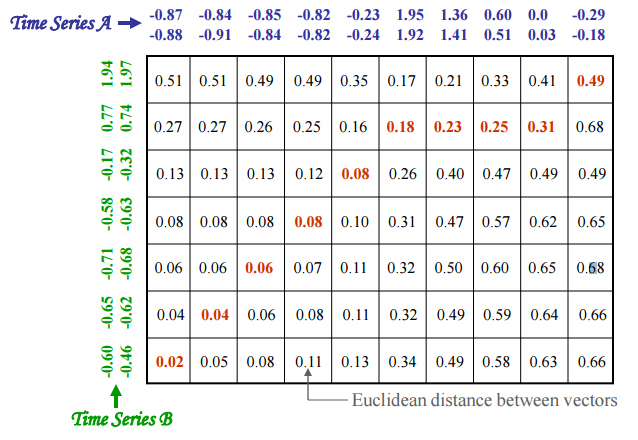
\includegraphics[width=0.8\textwidth]{./figure/trace_back.PNG}
  \caption{回溯法得到DTW路径示意图}\label{fig:6}
\end{figure}
回溯从累计距离矩阵的右上角开始,回溯的上一步是该方格左、下、斜下三个元素的最小值所在的方格,这样便能找到当前路径的上一步,通过不断这样地回溯,最终将到达路径的起始点,即得到DTW路径。

\subsection{带有权重系数的DTW方法}
对于DTW方法的路径走势,显然,路径总体斜向上游走,而不是呈阶梯形状游走更加合理。所以可以根据当前路径的走势,对路径的不同蜿蜒方向增加一个‘权重’,增加路径斜向上蜿蜒的可能性。此时,\ref{equ:4}中的最优化条件调整为:
\begin{equation}\label{equ:5}
  DTW(W) = \mathop {\min }\limits_W \left\{ {\frac{{\sum\limits_{k = 1}^K {d\left( {{w_{ki}},{w_{kj}}} \right) \cdot {\alpha _k}} }}{{\sum\limits_{k = 1}^K {{\alpha _k}} }}} \right\}
\end{equation}
${\sum\limits_{k = 1}^K {{\alpha _k}} }$是正则化项,可以被设定为常数$C$,因而\ref{equ:5}可以写成:
\begin{equation}\label{equ:6}
  DTW(W) = \frac{1}{C}\mathop {\min }\limits_W \left\{ {\sum\limits_{k = 1}^K {d\left( {{w_{ki}},{w_{kj}}} \right) \cdot {\alpha _k}} } \right\}
\end{equation}
$\alpha_k$表示第$k$步的权重系数,一般$\alpha_k$有以下几种取值:
\begin{enumerate}
  \item 对称形式:$\alpha_k = (i_k - i_{k-1})+(j_k - j_{k-1})$,也就是说若路径下一步是沿着斜向上方向游走,那么权重系数$\alpha_k = 2$,路径直向右或直向上游走,$\alpha = 1$,于是增加了路径斜向上游走的可能性。这种形式下,$C = m+n$。
  \item 非对称形式:
  \begin{itemize}
          \item $\alpha = (i_k - i_{k-1})$,这时$C = m$。
          \item $\alpha = (j_k - j_{k-1})$,这时$C = n$。
  \end{itemize}
  也就是说,在非对称情况下,路径朝上或朝右以及斜向游走,权重系数为2。
\end{enumerate}

对于带有权重系数的DTW方法,迭代公式只需要进行很小地调整。对于对称情形,迭代公式为:
\begin{equation}\label{equ:6}
  \gamma(i,j)=d(q_i,c_j)+\min \left( {\gamma \left( {i - 1,j} \right),\gamma \left( {i,j - 1} \right),\gamma \left( {i - 1,j - 1} \right)}+ d(q_i,c_j) \right)
\end{equation}
两种非对称情形的迭代公式分别为:
\begin{equation}\label{equ:7}
  \gamma (i,j) = d({q_i},{c_j}) + \min \left( {\gamma \left( {i - 1,j} \right) + d({q_i},{c_j}),\gamma \left( {i,j - 1} \right),\gamma \left( {i - 1,j - 1} \right) + d({q_i},{c_j})} \right)
\end{equation}
以及
\begin{equation}\label{equ:8}
  \gamma (i,j) = d({q_i},{c_j}) + \min \left( {\gamma \left( {i - 1,j} \right),\gamma \left( {i,j - 1} \right) + d({q_i},{c_j}),\gamma \left( {i - 1,j - 1} \right) + d({q_i},{c_j})} \right)
\end{equation}

在实际的DTW方法的应用中,可以根据实际情况,对路径的每一步赋予特定的权重,而这只需要在迭代公式上做很小的修改。

\section{DTW方法的加速技巧}
从上文中可以看到DTW方法的时间和空间复杂度都为$O(n^2)$,该节主要关注DTW方法的加速技巧。首先提出两种小技巧,最后引入能够将DTW时间和空间复杂度降低一个数量级的方法——FastDTW\cite{Salvador2007}。
\subsection{warp window}
虽然DTW方法能够对两序列中不同索引的元素进行对齐,但是直观上看,将两索引值相差过大的元素对齐在一起显然不合理。反映在距离矩阵上,也就是,路径不能偏离距离矩阵的对角线过大。基于此,可以定义warp window,使得路径蜿蜒在warp window所限定的区域之中。warp window如图\ref{fig:7} 所示。
\begin{figure}[h]
  \centering
  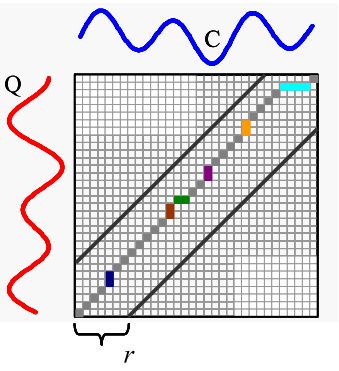
\includegraphics[width=0.4\textwidth]{./figure/warp_window.PNG}
  \caption{warp window示意图}\label{fig:7}
\end{figure}
不使用warp window,需要计算整个整个距离矩阵,也就是说,需要填充整个距离矩阵。利用warp window,只需要填充warp window所限定的、对角线周围的方格即可。所以引入warp window,在一定的程度上,降低了计算量。此外,因为引入warp window后,路径的蜿蜒更符合直观实际,因而理论上说,引入warp window能够提高DTW方法的精确度。
引入warp window后的DTW方法的伪代码如下所示:

\algsetup{linenosize = \tiny,
    linenodelimiter=.}
\begin{algorithm}[h]
\caption{Calculate DTW with warp window}
\begin{algorithmic}[1]
\small
\REQUIRE $Q:array[1..m], C:array[1..n]$, $w:$warp window
\ENSURE $DTW[m,n]$
\STATE $DTW := array[0..m,0..n]$
\STATE $w := max(w,\left| {m-n} \right|)$

\FOR {$i := 0$ to $m$}
\FOR {$j := 0$ to $n$}
\STATE $DTW[i,j] := inf$
\ENDFOR
\ENDFOR
\STATE $DTW[0,0] := 0$
\STATE
\FOR {$i := 1$ to $n$}
\FOR {$j := max(1,i-w)$ to $min(m,i+w)$}
\STATE $cost := d(Q[i],C[j])$
\STATE $DTW[i,j]:=cost+min(DTW[i-1,j],DTW[i,j-1],DTW[i-1,j-1])$
\ENDFOR
\ENDFOR
\end{algorithmic}
\end{algorithm}

与之前不带有warp window的DTW方法的主要不同在第$11$行中,通过控制$j$的取值范围来控制路径在距离矩阵中的蜿蜒范围。

\subsection{序列的分段平均表示法}
本节中的加快DTW计算的方法是从减小序列长度的角度出发的,序列的分段平均表示法\cite{Keogh2000} 是一种常用的有效减小序列长度的方法。首先介绍序列的分段平均表示法。
给定序列$X = x_1 x_2 \cdots x_n$,那么它的分段平均表示下的序列$\bar{X} = \bar{x_1} \bar{x_2} \cdots \bar{x_N}$,这里假定$n$能被$N$整除。其中$\bar{X}$的第$i$个元素是按照下面的计算式得到的:
\begin{equation}\label{equ:8}
  {\overline x _i} = \frac{N}{n}\sum\limits_{j = \frac{n}{N}\left( {i - 1} \right) + 1}^{\frac{n}{N}i} {{x_j}}
\end{equation}

\begin{figure}[h]
    \centering
    \begin{subfigure}[b]{0.45\textwidth}
        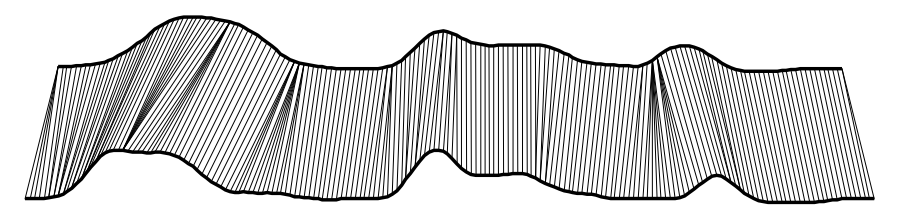
\includegraphics[width=\textwidth]{./figure/original.PNG}
        \caption{原始序列}
        \label{fig:subfig:original}
    \end{subfigure}
    ~ %add desired spacing between images, e. g. ~, \quad, \qquad, \hfill etc.
      %(or a blank line to force the subfigure onto a new line)
    \begin{subfigure}[b]{0.45\textwidth}
        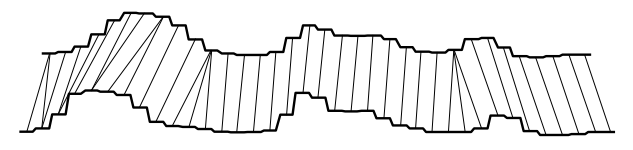
\includegraphics[width=\textwidth]{./figure/new.PNG}
        \caption{分段平均处理后的新序列}
        \label{fig:subfig:new}
    \end{subfigure}
    \caption{序列分段平均处理示意图}\label{fig:9}
\end{figure}
也就是说$\bar{X}$序列中的元素是对$X$序列中对应范围的元素求均值得到。经过序列分段平均处理后,再对新的较短的序列应用DTW方法,如图\ref{fig:9}所示。

在某些情况下,原始序列中的某些元素是序列中的噪声,经过序列分段平均处理,能从某种程度上消除序列噪声元素的影响,提取出序列特性。从这个角度看,对于某些序列,应用较为合适的序列分段平均处理,能够很大地减小序列长度,从而极大的加快DTW的计算,并且可以增加DTW方法的精度。

\subsection{FastDTW方法}
\subsubsection{FastDTW方法简介}
上面介绍的两种方法只能从DTW的实际应用经验上加快DTW方法的计算,本节引入一种新的能够从算法的角度有效地把DTW方法的时间以及空间复杂度从$O(n^2)$降低到$O(n)$的方法——FastDTW\cite{Salvador2007}。
FastDTW的思想是首先降低距离矩阵的分辨率,在较低分辨率下,得到DTW路径,然后对较低分辨率的路径所经过的方格,得到在较高分辨率下路径所能够走的方格的限制。算法主要包括以下三个关键步骤:
\begin{enumerate}
  \item \textbf{粗化}:首先利用上面所提到的序列分段平均表示法,得到较短的序列。假设较短序列长度为原序列长度的$\frac{N}{n}$,那么这些短序列构成的距离矩阵的宽度为原距离矩阵宽度的$\frac{N}{n}$,也就是说,现在得到$\frac{1}{\frac{n}{N}}$分辨率的距离矩阵。
  \item \textbf{投影}:即找到低分辨率下的DTW路径。
  \item \textbf{细化}:由低分辨率下DTW路径所经过的距离矩阵方格,找到较高分辨率下这些方格的对应方格,便找到高分辨率下DTW路径的约束。
\end{enumerate}
FastDTW方法的示意图如\ref{fig:10}所示。
\begin{figure}[h]
  \centering
  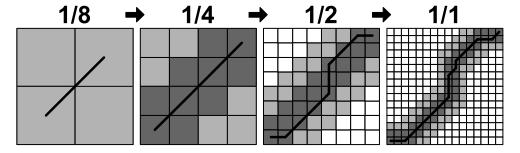
\includegraphics[width=0.7\textwidth]{./figure/FastDTW.PNG}
  \caption{FastDTW示意图}\label{fig:10}
\end{figure}

以图中的$\frac{1}{2}$分辨率到$\frac{1}{1}$分辨率为例。首先$\frac{1}{2}$低分辨率是$\frac{1}{1}$高分辨率下,通过对原始序列进行分段平均处理后得到的。在$\frac{1}{2}$分辨率下可以得到如图所示的路径,路径周围黑色的方块是该分辨率下路径所走过的区域。在将分辨率调高到$\frac{1}{1}$分辨率后,$\frac{1}{2}$分辨率下得到的黑色方块区域也相应地投影到$\frac{1}{1}$分辨率中,即是$\frac{1}{1}$分辨率中的黑色区域。但是在实际的操作中,为了使得得到的路径更为精确,这是会人为地设定一个参数:半径$r$,它是一个倍率,表示将黑色区域扩大了多少倍。$\frac{1}{1}$分辨率下的黑色区域外围的灰色区域即是加入半径参数后对黑色区域的扩大,在该图所示的情况下,$r=1$,在$\frac{1}{1}$分辨率的距离矩阵中,路径蜿蜒区域被限定在黑色和灰色区域中。

在实际的FastDTW操作中,首先会把分辨率调低到一个合理的水平,然后逐步调高分辨率,每种分辨率下均能得到一条路径,最终将得到$\frac{1}{1}$分辨率下的路径。FastDTW对于每一种分辨率取最优路径,但是最终得到的不一定是和原始DTW方法相同的最优路径,因为从低分辨率路径得到的高分辨率情形下的路径限制方格,只是高分辨率中,路径最有可能经过的方格,真实的最优路径可能会‘突破’这些限制方格,所以FastDTW方法最终所得到的路径可能会和原始DTW路径有所不同。增大半径$r$,会降低路径约束,使得FastDTW路径和原始DTW路径更为接近,但增加半径会使得需要填充的距离矩阵的方格更多,从而增加了计算量。

\subsubsection{FastDTW方法的时间、空间复杂度分析}
首先计算FastDTW方法总共需要计算距离矩阵的元素,直观上看,也就是需要填充多少距离矩阵的方格。首先,考虑从$\frac{1}{2}$分辨率到$\frac{1}{1}$分辨率需要填充方格数目最多的情况,如图\ref{fig:11}所示:
\begin{figure}[h]
  \centering
  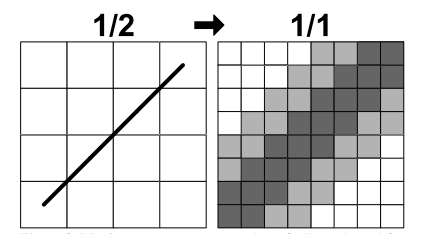
\includegraphics[width=0.4\textwidth]{./figure/evaluation.PNG}
  \caption{最大填充方格示意图}\label{fig:11}
\end{figure}

$\frac{1}{1}$分辨率的图示中,黑色和灰色的区域都需要填充,因而在$\frac{1}{1}$分辨率情形下,需要填充的最大方格数目上限为:$3N + 2\cdot (2Nr) = N(4r+3)$。 因为分辨率会有$\frac{1}{1},\frac{1}{2},\frac{1}{2^2},\frac{1}{2^3},\cdots$这些,因而在所有分辨率下总共需要填充的方格数目为:
\begin{equation}\label{equ:9}
  N\left( {4r + 3} \right) + \frac{N}{2}N\left( {4r + 3} \right) + \frac{N}{{{2^2}}}N\left( {4r + 3} \right) + \frac{N}{{{2^3}}}N\left( {4r + 3} \right) \cdots  = 2N\left( {4r + 3} \right)
\end{equation}

而时间复杂度由下面三部分组成:
\begin{enumerate}
  \item 需要计算的方格数目。刚刚已经计算得到,是$2N\left( {4r+3}\right)$。
  \item 计算得到不同的分辨率。对于一段序列(长度为$N$)来说,不同分辨率下需要的时间复杂度之和为:$N + \frac{N}{2} + \frac{N}{2^2} + \frac{N}{2^3} + \cdots = 2N$,因为有两段序列,因而这部分的总时间复杂度为$4N$。
  \item 回溯得到不同分辨率下的路径。$\frac{1}{1}$分辨率下,路径长度最多为$2N$,也就是说最多需要比较$2N$次。所以所有分辨率下,回溯得到路径的时间复杂度是:$2N + \frac{2N}{2} + \frac{2N}{2^2} + \frac{2N}{2^3} + \cdots = 4N$。
\end{enumerate}
将这三项加起来,可得FastDTW方法的时间复杂度为:$N(8r+14)$。
可以看到,FastDTW是线性时间复杂度。

再来估计空间复杂度。空间复杂度由下面三部分组成:
\begin{enumerate}
  \item 存储不同分辨率下的序列。因为不同分辨率下的序列长度分别为$N,\frac{N}{2},\frac{N}{2^2},\frac{N}{2^3},\cdots$,而有两条序列,因而存储不同分辨率下序列的空间复杂度为$4N$。
  \item 存储不同分辨率下的距离矩阵。前面已经估计到,总共需要填充的距离矩阵方格数目为$N(4r+3)$。
  \item 存储路径。前面也已经说明,存储路径的空间复杂度的上限为$4N$。
\end{enumerate}
因而FastDTW方法总的空间复杂度为:$N(4r+11)$。同样地,FastDTW方法也为线性空间复杂度。
当序列的长度比较小,也就是$N$比较小时,$N(8r+14)$以及$N(4r+11)$的复杂度与$N^2$相比并没有优势,$N$很大时,$N(8r+14)$以及$N(4r+11)$将远远小于$N^2$,因而,对于长序列,FastDTW的时间、空间复杂度将远远优于原始DTW方法。

\section{实验结果}
\subsection{实验1}
首先简单地使用人造数据比较欧几里得距离和DTW距离的分类精确度。实验有四类,每一类中训练集、测试集均都有四个序列,序列的长度均为100,相邻类的两序列都有间隔参数$interval$,序列是在相邻类间隔为$interval$的常数序列中增加随机噪声而产生的,现通过1NN的方法对测试集中的序列分类,即将测试集中的序列归类到距离最近的那个序列所属的类,然后和测试集序列的$label$相比较,计算得到分类精确度。最终的分类精确度是上面的数据集分类100次得到的平均精确度。

将间隔参数$interval$从0变化到2,可以得到相应的欧几里得距离和DTW距离的分类精确度曲线,如图\ref{fig:12} 所示。
\begin{figure}[h]
  \centering
  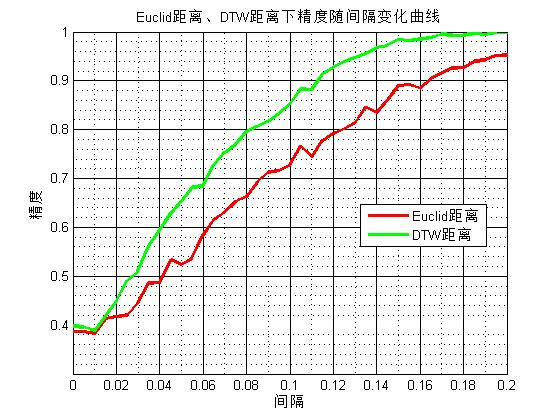
\includegraphics[width=0.6\textwidth]{./figure/interval.jpg}
  \caption{Euclid、DTW距离下分类精确度随间隔变化曲线}\label{fig:12}
\end{figure}
实验所得到的精确度曲线中,大部分情况下,DTW距离的分类精度曲线都在欧几里得距离的分类精度曲线上面,这说明了DTW距离相对于传统欧几里得距离的优越性。

\subsection{实验2}
实验1是使用人造数据进行实验,实验2把数据换为权威的官方数据。UCR Time Series Classification Archive是加州大学河边分校相关研究人员收集的时间序列数据集\cite{UCR_data},现采用其中的部分数据集,使用DTW以及欧几里得距离进行分类,得到结果如表 所示。

\begin{table}[ht]
\centering
\begin{tabular}{|c|c|c|c|c|c|c|c|}
    \hline
    % after \\: \hline or \cline{col1-col2} \cline{col3-col4} ...
    name & Gun\_Point & Plane & StrawBerry \\
    \hline
    lasses & 2 & 7 & 2 \\
    \hline
    training set size  & 50 & 105 & 370 \\
    \hline
    test set size  & 150 & 105 & 613 \\
    \hline
    sequence length & 150 & 144 & 235 \\
    \hline
    error rate (Euclid) & 0.086667 & 0.038095 & 0.06199 \\
    \hline
    error rate (DTW) & 0.12 & 0 & 0.066884 \\
    \hline
\end{tabular}
\newline
\newline
\newline
\begin{tabular}{|c|c|c|c|c|c|c|c|}
    \hline
    % after \\: \hline or \cline{col1-col2} \cline{col3-col4} ...
    name & Computers & Trace & FaceFour & WordsSynonyms\\
    \hline
    lasses & 2 & 4 & 4 & 25  \\
    \hline
    training set size & 250 & 100 & 24 & 267  \\
    \hline
    test set size & 250 & 100 & 88 & 638  \\
    \hline
    sequence length & 720 & 275 & 350 & 270  \\
    \hline
    error rate (Euclid) & 0.424 & 0.24 & 0.21591 & 0.38245 \\
    \hline
    error rate (DTW) & 0.332 & 0.01 & 0.15909 & 0.32445  \\
    \hline
\end{tabular} \caption{UCR数据集实验结果 } \label{tab:1}
\end{table}

从实验结果中的两个表格可以看出,在大多数情况下,DTW方法的分类精确度都要高于传统的欧几里得距离。

\subsection{实验3}
上文已经说过,通过定义warp window,不但能够减小计算量,而且能够在某种程度上增大分类精度。现在对于部分UCR数据集以及$interval = 0.875$时的人造数据集,从0到1变化warp window的比例,得到各种比例下的分类精度,得到分类精度曲线,如图\ref{fig:13} 所示。
\begin{figure}[h] \centering
    \begin{subfigure}[t]{0.4\linewidth}
        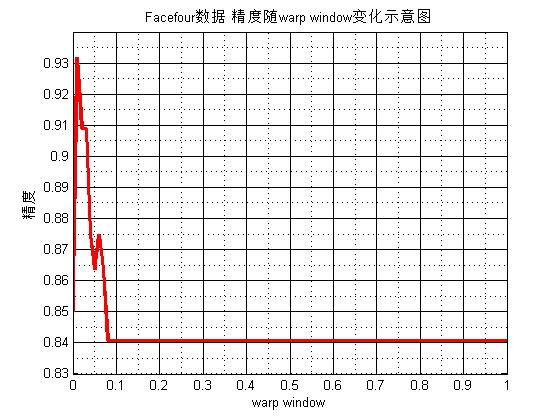
\includegraphics[width=\linewidth]{./figure/facefour.jpg}
        \caption{facefour数据} \label{fig:subfigure:1}
    \end{subfigure} %
    \quad
    \begin{subfigure}[t]{0.4\linewidth}
        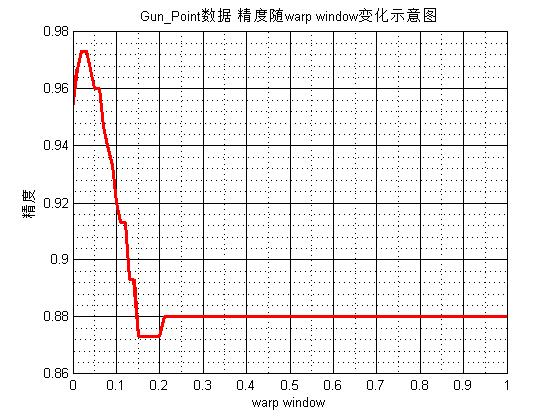
\includegraphics[width=\linewidth]{./figure/gun_point.jpg}
        \caption{gun\_point数据} \label{fig:subfigure:2}
    \end{subfigure}

    \begin{subfigure}[t]{0.4\linewidth}
        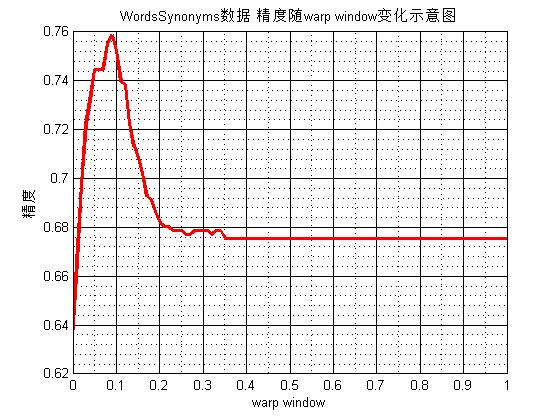
\includegraphics[width=\linewidth]{./figure/WordsSunonyms.jpg}
        \caption{WordsSunonyms数据} \label{fig:subfigure:3}
    \end{subfigure}
    \quad
    \begin{subfigure}[t]{0.4\linewidth}
        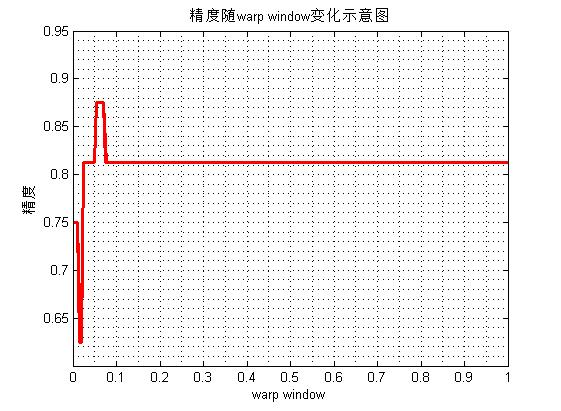
\includegraphics[width=\linewidth]{./figure/accuracy_warp_window.jpg}
        \caption{interval为0.875时的人造数据} \label{fig:subfigure:4}
    \end{subfigure}
    \caption{不同数据集分类精度随warp window变化曲线}
    \label{fig:13}
\end{figure}
从分类精度随warp window变化曲线可以看出,较小的warp window(大部分情况下小于10\%)会提升分类精度。事实上,很多文献\cite{UCR_data} \cite{Ratanamahatana2005} 也说明这点。

\chapter{Shapelets方法}
上面介绍的DTW方法是从构造衡量两序列距离的角度分析,而本章通过序列最具特征子序列来完成分类。
\section{Shapelets简介以及定义}
在日常的生活中,人们在对一个物体进行分类的时候,会根据这一类物体所具有的共同特征,比如我们想要区分一支笔是铅笔还是钢笔,我们只需根据笔尖的种类即可,笔尖带有圆珠,那么这支笔就是圆珠笔,笔尖中心有缝隙,那么这支笔就是钢笔。也就是说,对笔分类时,我们仅仅需要利用最能代表笔特征的部位——笔头即可。同样地,  对于某些序列数据来说,我们也可以利用这种共同特征来对序列数据分类,这种体现共同特征的,序列集合中的某序列的子序列就是Shapelets\cite{Ye2009}。

一般而言,Shapelets方法有以下三点好处:
\begin{itemize}
  \item 得到可解释的结果:应用Shapelets方法的时候,结果中将包含一类序列的共同特征,这些共同特征将有助于对分类结果进行解释。
  \item 对于一些数据而言分类的结果更为精确。Shapelets方法和大多数方法的不同之处在于,Shapelets方法考虑的是序列的局部特征,而其他方法多考虑序列整体,这些方法比较容易受到序列中的无用部分以及序列中的噪声、失真等影响。例如把笔杆也考虑进分类中,那么分类结果必不如只考虑笔尖精确。
  \item Shapelets方法的时间复杂度比较低。在得到Shapelets的情况下,分类的时间复杂度为$O(ml)$,$m$是待分类序列的长度,$l$是Shapelets的长度。因为Shapelets是序列片段,因而一般情况下,$l$都比较小。
\end{itemize}

一般可以借助信息增益来找到Shapelets,给定顺序序列$T = t_1,t_2,\cdots ,t_m$,下面来逐步地给出Shapelets的定义。

\begin{mydef}
\emph{子序列.}序列$T$的长度为$l$的子序列$S$是由$T$中$l$个连续元素所组成的,$S = t_p,t_{p+1},\cdots,t_{p+l-1} \quad p+l-1 \leq m$。
\end{mydef}

\begin{mydef}
\emph{长度为$l$的子序列集合.} 定义 $S_p^l = {t_p},{t_{p + 1}}, \cdots ,{t_{p + l - 1}}$是$T$的起始点为$t_p$,长度为$l$的子序列。那么$T$的所有长度为 $l$ 的子序列集合是 $\bm{S}_T^{\left| S \right|} = \left\{ {S_p^l,1 \le p \le m - l + 1} \right\}$。
\end{mydef}

\begin{mydef}
\emph{子序列$S$和长序列$T$之间的距离$SubSeqDist(S,T)$.}定义$SubSeqDist\left( {T,S} \right) = \min \left( {Dist\left( {S,{S^{'}}} \right),{S^{'}} \in \bm{S}_T^{\left| S \right|}} \right)$ ,即$S$和 $T$之间的距离是$S$和$T$中所有等长子序列之间距离的最小值,如图\ref{fig:14}所示。
\end{mydef}

\begin{figure}[h]
  \centering
  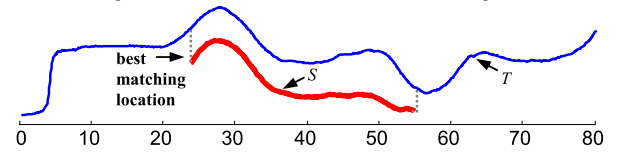
\includegraphics[width=0.6\textwidth]{./figure/subdist.PNG}
  \caption{子序列和长序列距离示意图}\label{fig:14}
\end{figure}

之所以把$S$和$T$之间的距离定义成$S$和$T$的子序列之间的距离,是因为Shapelets方法是对序列子序列比较的方法。

后文中将要看到,Shapelets会将不同的类给分开,可以通过信息论中的信息增益来衡量这种分开的好坏。

\begin{mydef}
\emph{熵.}假定序列集合$\bm{D}$由两类$A$,$B$组成,比例分别为$p(A)$和$p(B)$,那么$\bm{D}$的熵的定义是$I(\bm{D}) = -p(A)log(p(A))-p(B)log(p(B))$。
\end{mydef}

有了熵的定义,那么就能得到Shapelets分类前后的信息增益。

\begin{mydef}
    \emph{信息增益.}特定的划分策略$sp$将数据集$\bm{D}$划分成两个子序列集$\bm{D_1}$、$\bm{D_2}$,那么信息增益定义为:
    \begin{equation}\label{equ:10}
      Gain\left( {sp} \right) = I\left( \bm{D} \right) - \mathop I\limits^ \wedge  \left( \bm{D} \right)
    \end{equation}
    也就是:
    \begin{equation}\label{equ:11}
      Gain\left( {sp} \right) = I\left( D \right) - f\left( {{D_1}} \right)I\left( {{D_1}} \right) + f\left( {{D_2}} \right)I\left( {{D_2}} \right)
    \end{equation}
\end{mydef}

如图\ref{equ:entropy}所示,序列集$\bm{D}$中有10个序列,包括两类,分别用红色和蓝色表示,每类的序列数目分别为4和6,计算Shapelets候选序列和$\bm{D}$中序列距离,按照大小关系排列在坐标轴上,如图所示的最优分割点的情况下,信息增益为:
\begin{equation}\label{equ:entropy}
  \left[ { - \frac{6}{{10}}\log \left( {\frac{6}{{10}}} \right) - \frac{4}{{10}}\log \left( {\frac{4}{{10}}} \right)} \right] - \left[ {\frac{5}{{10}}\left[ { - \frac{5}{5}\log \left( {\frac{5}{5}} \right)} \right] + \frac{5}{{10}}\left[ { - \frac{4}{5}\log \left( {\frac{4}{5}} \right) - \frac{1}{5}\log \left( {\frac{1}{5}} \right)} \right]} \right] = 0.482
\end{equation}
\begin{figure}
  \centering
  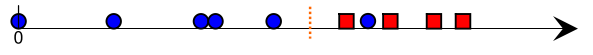
\includegraphics[width=0.8\linewidth]{./figure/entropy.PNG}
  \caption{信息增益计算的示意图}\label{equ:entropy}
\end{figure}

需要说明的是Shapelet是序列集$\bm{D}$中所有子序列中的某个,那么Shapelets候选集就是$\bm{D}$的所有子序列。

\begin{mydef}
    \emph{最优分隔点($OSP$).}数据集$\bm{D}$中包含两类序列$A$和$B$。对于Shapelets候选序列$S$,根据上面的距离的定义可以得到$S$与$\bm{D}$中所有序列之间的距离,选择距离阈值$d_{th}$,可以将$\bm{D}$中的序列分为$\bm{D}_1$和$\bm{D}_2$两类,$\bm{D_1}$中的序列$T_{1,i}$满足$SubSeqDist(S,T_{1,i}) \le d_{th}$,$\bm{D_2}$中的序列$T_{2,i}$满足$SubSeqDist(S,T_{2,i}) \ge d_{th}$。最优分隔点是所有分割点$d_{th}^{'}$中,使得信息增益最大的那个分割点:
    \begin{equation}\label{equ:12}
      Gain\left( {S,{d_{OPS\left( {D,S} \right)}}} \right) \ge Gain\left( {S,d_{th}^{'}} \right)
    \end{equation}
\end{mydef}

有了以上这些定义,最后将给出Shapelets的定义。

\begin{mydef}
    \emph{Shapelets.}给定含有两类序列的序列集合$\bm{D}$,$Shapelet(\bm{D})$是$\bm{D}$的子序列,满足对于$\bm{D}$的所有子序列$S$:
    \begin{equation}\label{equ:13}
        Gain\left( {Shapelet\left( D \right),{d_{OPS\left( {D,Shapelet\left( D \right)} \right)}}} \right) \ge Gain\left( {S,{d_{OPS\left( {D,S} \right)}}} \right)
    \end{equation}
\end{mydef}

也就是说,在最优分割的情况下,利用Shapelet对序列集合进行分割,信息增益最大。

\section{Shapelet计算以及加速方法}
\subsection{Shapelet的计算}
利用Shapelets进行序列分类,首先需要找到序列集合的Shapelets,算法如下。

\algsetup{linenosize = \tiny,
    linenodelimiter=.}
\begin{algorithm}[h]
\caption{Brute force algorithm for finding shapelet}
\begin{algorithmic}[1]
\small
\REQUIRE dataset \textbf{$D$},\emph{MAXLEN},\emph{MINLEN}
\ENSURE bsf\_shapelet

\STATE candidates := GenerateCandidates(\textbf{$D$},\emph{MAXLEN},\emph{MINLEN})
\STATE bsf\_gain := 0
\FOR { S in candidates}
\STATE gain:=CheckCandidate(D,S)
\IF {gain>bsf\_gain}
\STATE bsf\_gain :=gain
\STATE bsf\_shapelet :=S
\ENDIF
\ENDFOR
\end{algorithmic}
\end{algorithm}

伪代码的第一行是构造Shapelets候选集,该步中,Shapelets候选集是长度介于$MINLEN$,$MAXLEN$之间的所有子序列。然后遍历候选集中的所有候选序列,能够在最优分割情况下使得信息增益最大的候选序列即是序列集合的Shapelet。

\subsection{Shapelet计算的加速方法}
在寻找Shapelet的过程中,需要遍历序列集所有的子序列,那么候选序列的总共数目将特别地大,而且在计算候选序列和原长序列的距离时,需要遍历原长序列中和候选序列等长的子序列,寻找最优分隔点也需要很大的计算量,所以寻找Shapelet的计算量特别大,下面介绍能够减小计算量的两种方法。

\subsubsection{$SubSeqDist$计算的提早舍弃}
对于Shapelets候选序列$S$和原始序列$T$,假设当前是取出$T$的子序列$S^{'}$与$S$求距离。计算$S$与$S^{'}$之间的距离,是按索引从小到大逐步计算的,我们可以把之间计算得到的最小距离给记录下来,当索引值推进到$S$和$S^{'}$的某一步时,比较当前的距离和之前已记录的最小距离之间的大小,如果当前的距离比记录的最小距离大,那么就没有必要再拿$S^{'}$和$S$比较下去,那么选择$T$的下一个子序列和$S$求距离。如图\ref{fig:15} 所示。
\begin{figure}[h]
  \centering
  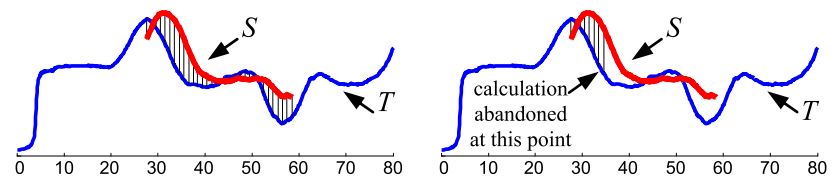
\includegraphics[width=0.75\linewidth]{./figure/subdistance.PNG}
  \caption{计算候选序列和原始序列距离时的提早舍弃}\label{fig:15}
\end{figure}

\subsubsection{计算熵的时候的提早舍弃}
还是接着图\ref{equ:entropy}进行说明。对于另一个Shapelets候选序列$\bar{S}$,假设当前已经计算了$\bar{S}$和$\bm{D}$中的5个序列(2个红色序列,3个蓝色序列)之间的距离,并按照大小顺序排列好,如图\ref{fig:16}所示。
\begin{figure}[h]
  \centering
  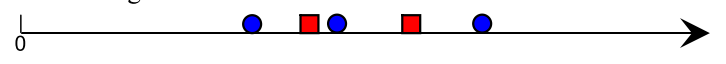
\includegraphics[width=0.6\linewidth]{./figure/Entropy2.PNG}
  \caption{候选序列与序列集中5个序列距离大小排列情况}\label{fig:16}
\end{figure}

对于下面的5个序列,当3个蓝色序列在最左边、2个红色序列在最右边或者3个蓝色序列在最右边、2个红色序列在最左边时,能获得的信息增益最大,如图\ref{fig:17} 所示,可以计算这种最大信息增益与之前记录的最大信息增益的大小关系,如果小于之前记录的最大信息增益,那么说明当前的Shapelets候选序列肯定不是最终的Shapelet,所以应该选择Shapelets候选集中的下一个候选序列进行计算。

\begin{figure}[h]
  \centering
  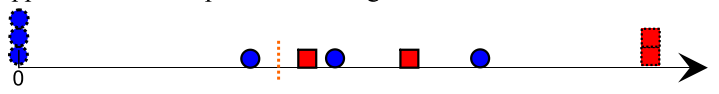
\includegraphics[width=0.6\linewidth]{./figure/Entropy3.PNG}
  \caption{使得熵最大的极端情况示意图}\label{fig:17}
\end{figure}

在得到序列集的Shapelet后,比较待分类序列和Shapelet之间的距离,根据距离远近,对待分类序列进行分类。

% 致谢
\begin{thanksfor}
    这次的毕业论文设计总结是在我的指导老师徐林莉老师亲切关怀和悉心指导下完成的。从毕业设计选题到设计完成,徐老师给予了我耐心指导与细心关怀,在此表示感谢。徐老师有严肃的科学态度,严谨的治学精神和精益求精的工作作风,这些都是我所需要学习的!感谢研究组里提供的优良的科研资源,这让我享受到了难忘的学习时光,感谢师兄们的指导。另外,也特别感谢崔元顺同学提供的latex模板。
\end{thanksfor} 

%参考文献
\phantomsection%生成该页的链接
\addcontentsline{toc}{chapter}{\bibname}
\bibliographystyle{XDUbib}%plain ieeetr
\bibliography{ThesisFiles/RefFile}%在正文中必须引用,才能显示对应的参考文献

% 附录部分
\appendix
  

\end{document}

